\chapter{The Higgs Bosons and the MSSM}
This chapter is devoted to introduce the the Minimal Supersymmetric 
extension of the Standard Model (MSSM) whit focus on  its Higgs sector.
In section... introduction is given based on~\cite{Altarelli}, 


\clearpage

\section{The Standard Model of Particle Physics and its Limitations}
\subsection{Overview of the SM}
The Standard Model (SM) of particle physics is a theory aimed to describe and quantitatively predict
the phenomenology of foundamental interaction. At ``microscopic''  level all the phenomenology of matter and 
radiation can be understood in terms of three classes of foundamental interactions, which are the strong, the electromagnetic
and the weak interactions, the gravitational force is instead negligible in atomic and nuclear physics (quantum effects in gravity are
expected to become important at energies corresponding to the Planck mass $E \sim M_{planck} c^2 \sim 10^{19}$ GeV).
All these interactions (with the exception of gravity) are described by a local relativistic quantum field theory.
To each particle, described as pointlike, is associated a field with suitable
(depending on the particle spin) transformation properties under the Lorentz group (the
relativistic space-time coordinate transformations). The description
of all these particle interactions is based on a common principle: ``gauge'' invariance. A
gauge symmetry is invariance under transformations that rotate the basic internal degrees of freedom but
 with rotation angles that depend on the space-time point.

The SM is a gauge field theory based on the symmetry group $SU(3)_c \otimes SU(2)_L \otimes U(1)_Y$. This group has $8+3+1=12$
generators with a non trivial commutator algebra. The electromagnetic and weak interactions (EW) are described \cite{} by the 
$SU(2)_L \otimes U(1)_Y$ symmetry group, while the $ SU(3)_c$ is the colour group of the theory of strong interactions (QCD)~\cite{}.
To each generator of the symmetry group is associated a vector boson which act as mediator of the correspondig interactions.
Eight gluons are associated to the $ SU(3)_c$ colour generators, while for $SU(2)_L \otimes U(1)_Y$ there are four gauge bosons $W^{\pm}$,
$Z^0$ and $\gamma$. Of these, only the gluons and the photon are massless since the symmetry induced by the other three generators is
spontaneusly broken. In the SM the spontaneus symmetry breacking is realized by the Higgs mechanism~\cite{}, the Higgs particle has 
been recently found at the LHC with $m_H \sim 125$ GeV \cite{} representing one of the major mailstone of particle physics.
The Higgs boson acts as mediator of a new class of interactions that, at tree level, are coupled in proportion to the particle masses.

The fermionic (all of spin 1/2) matter fields of the SM are quarks and leptons. 
Quarks  are subject to all SM interactions, each type of quark is a colour triplet and carries 
electroweak charges, in particular electric charges $+2/3$ for up-type quarks and $-1/3$
for down-type quarks.  Leptons are colourless
but have electroweak charges, in particular electric charges $-1$ for charged leptons $e$, $\mu$ and $\tau$ (opposite sign charge 
is intended for respective anti-particle)  and charge 0 for neutrinos $\nu_e$, $\nu_{\mu}$ and $\nu_{\tau}$.
Qarks and leptons are grouped in three  ``generations'' with equal quantum numbers but different masses.

\subsection{Precision Test and Limitation of the SM}

Precision tests of the SM has been performed over a wide range of energies in experiment in the last several decades,
Precision tests~\cite{precisiontest} of the standard electroweak theory performed at LEP, SLC and Tevatron~\cite{smtest}, 
has confirmed the couplings of quark and leptons to the weak gauge bosons $W^{\pm}$  and $Z$ are indeed
precisely those prescribed by the gauge symmetry. The accuracy of a few per-mille for these
tests implies that, not only the tree level, but also the structure of quantum corrections has
been verified. Several other experimental results~\cite{pdg} rare decays and the anomalus magnetic moment of the muon
provide a test for low-energies of the standard model.

%However 
%In spite of this success, the conceptual situation with the
%standard model is unsatisfactory for quite a few deficiencies:
%– the smallness of the electroweak scale v ∼ 246GeV << MPl (the ‘hierarchy problem’);
%– the large number of free parameters (gauge couplings,
%vacuum expectation value, MH, fermion masses,
%CKM matrix elements), which are not predicted but have
%to be taken from experiments;
%– the pattern that occurs in the arrangement of the
%fermion masses;
%– the missing way to connect to gravity.
%
%-Dark matter
%
%-neutrino masses

 
\section{The Minimal Supersymmetric Standard Model}
\subsection{Introduction}
Supersymmetry (SUSY) was first introduced since it offer a natural way to solve the hierarchy problem....\cite{}
This is achieved by introducing a symmetry transformation that relates bosons with fermions. The SUSY generators $\mathcal{Q}$ 
transforms fermion into bosons and vice versa:
\begin{equation}
\mathcal{Q}|\text{Fermion}\rangle = |\text{Boson}\rangle, ~ ~ ~ \mathcal{Q}|\text{Boson}\rangle = |\text{Fermion}\rangle
\end{equation}
This is suggesting that in a supersymmetric extesion of the SM \cite{page7Martins} each of the known foundamental particles 
is in either a chiral or gauge ``supermultiplet'' and must have a superpartner with spin differing by 1/2 unit.
Fermions since the left-handed and right-handed component transform differently under gauge transformations also their superpartner 
should maintain this property, the name of the superpartner of the quarks and leptons are made by adding an ``s'' to the SM name, standing for scalar.
Accordingly, the gauge bosons related to the generator of the group $SU(3)_c \otimes SU(2)_L \otimes U(1)_Y$ should also have a spin 1/2 partner,
whose name will be made by adding a ``ino'' at the end of the SM name. The symbol of superpartners is defined by adding a ($\tilde{ ~ }$) to the SM symbol.

The  Minimal Supersymmetric extension of the Standard Model  (MSSM)~\cite{page11Djuadi}, is defined by requiring the minimal gauge group (i.e., the SM one)
and the minimal particle content: three generation of fermions (without right-handed neutrinos), gauge bosons and two Higgs doublet, 
each with its superpartners. Tables~\ref{tab:chiralsup} and~\ref{tab:gaugesup} summarize chiral and gauge supermultiplets in the MSSM.
This guys will mix to form neutralino and chargino....
\begin{table}
\begin{center}
\renewcommand{\arraystretch}{1.5}
\begin{tabular}{c|ccc}
\hline%\noalign{\smallskip}
Names 			&Supermultiplets	&	Spin 1/2  		& Spin 0 \\%[0.1cm]
\hline%\noalign{\smallskip}		
quark, squarks		& $Q$ 			&	$(u_L ~ d_L)$		& $( \tilde{u}_L ~ \tilde{d}_L)$ \\%[0.1cm]
($\times$ 3 families)	& $\bar{u}$		& 	$u_R^{\dagger}$ 	& $\tilde{u}_R^*$ \\%[0.1cm]
			& $\bar{d}$		& 	$d_R^{\dagger}$ 	& $\tilde{d}_R^*$ \\%[0.1cm]
\hline%\noalign{\smallskip}
leptons, sleptons	& $L$			&   	$(\nu ~ e_L)$ 		&  $( \tilde{\nu} ~ \tilde{e}_L)$\\%[0.1cm]
($\times$ 3 families)	& $\bar{e}$		&	$e_R^{\dagger}$         & $\tilde{e}_R^*$ \\%[0.1cm]
\hline%\noalign{\smallskip}
higgsinos, Higgs	& $H_1$			&	$( \tilde{H}_1^0 ~ \tilde{H}_1^-)$  &	$( H_1^0 ~ H_1^-)$ \\%[0.1cm]	 
			& $H_1$			&	$( \tilde{H}_2^+ ~ \tilde{H}_2^0)$  &	$( H_2^+ ~ H_2^0)$ \\%[0.1cm]	 
\hline
\end{tabular}
\caption{This table is based on~\cite{SusyPrimer} and summarize the chiral supermultiplets in the Minimal Supersymmetric Standard Model. The spin-0 fields are complex scalars
	and the spin-1/2 are left-handed two-component Weyl fermions.}
\label{tab:chiralsup}
\end{center}
\end{table}

\begin{table}
\begin{center}
\renewcommand{\arraystretch}{1.5}
\begin{tabular}{c|cc}
Names			& Spin 1 		&	Spin 1/2 \\
\hline
gluon, gluino		& $g$			& $\tilde{g}$	\\
W bosons, winos		& $W^{\pm}$ $W^0$	& $\tilde{W}^{\pm}$ $\tilde{W}^0$ \\
B boson, bino		& $B^0$			& $\tilde{B}^0$ \\
\hline
\end{tabular}
\caption{This table is based on~\cite{SusyPrimer} and summarize the gauge supermultiplets in the Minimal Supersymmetric Standard Model.}
\label{tab:gaugesup}
\end{center}
\end{table}

\subsubsection{$R$-parity conservation}
The MSSM also requires a discrete and multiplicative symmetry called $R$-parity~\cite{djuadi12}, this symmetry assures barion and lepton number 
conservation and it is defined as follows:
\begin{equation}
R_p = (-1)^{2s+3B=L}
\end{equation}
where $L$ and $B$ are lepton and barion numbers and $s$ stands for the spin quantum number. R-parity quantum numbers has value $+1$ for ordinary
SM particles and $-1$ for their superpartners. This symmetry was first introduced to overcome the problem of instability of the proton,
lepton and barion number violation leads, in many cases, 
to unstable proton with life-time shorter than the experimental lower limit. However the conservation of $R$-parity has also other important 
fenomenological consequences, SUSY particle are always produced in pairs and in their decay there is always an odd number of SUSY particle, 
and the lightest SUSY particle is stable, providing a good candidate for dark matter.


\subsubsection{The Soft SUSY Breaking}
In case the Supersymmetry is an exact symmetry of nature, the bosonic fields and the corrispective fermion fields should have the same mass 
and quantum numbers, except for the spin. However, the particle spectrum of SUSY has not yet been observed, suggesting that these particle
 should have an higher mass than their SM superpartners. 
To achieve SUSY-breaking in a way which does not reintroduce the quadratic divergences to the Higgs mass squared, a so called ``soft-SUSY-breaking''
term is introduced~\cite{djuadipage5orBetterPage12}, this term explicitly break SUSY introducing ad hoc the mass terms for Higgs, gauginos and
sferions, furthermore  trilinear coupling terms between sfermions and Higgs bosons are introduced. In general, if intergenerational mixing and 
complex phases are allowed, the soft-SUSY-breaking terms will introduce a huge number of unknown parameters $\mathcal{O}(100)$~\cite{djuadiPage5}.
However, in absence of phases and  mixing, and if obey to a set of boundary conditions~\cite{djuadi5}, only few new parameters are introduced.




\subsection{The Higgs Sector in the MSSM }
In the MSSM two doublets of complex scalar field of opposite hypercharge are required to break the electroweak symmetry, 
this requirement is motivated by the needs to generate  masses separately to isospin up-type fermion and down-type fermions~\cite{djouadiP21}
and to cancel chiral anomalies that otherwise would spoil the renormalizability of the theory~\cite{djouadiP21}. The two Higgs doublet then are:
\begin{equation}
H_1 = \binom{H_1^0}{H_1^-} ~ ~ \text{with } Y_{H_1} = -1, \quad \quad H_2 = \binom{H_2^+}{H_2^0} ~ ~ \text{with } Y_{H_2} = +1  
\end{equation}
In analogy with the SM, a similar Higgs mechanism is employed in the MSSM~\cite{djuadiP22},  requiring that the minimum 
of the Higgs potential breaks $SU(2)_L \otimes U(1)_Y$ group while preserving the electromagnetic symmetry $U(1)_Q$.
the  to break electroweak symmetry. The neutral components of the 
two Higgs field acquire vacuum expectation values:
\begin{equation}
\langle H_1^0 \rangle = \frac{v_1}{\sqrt{2}}, \quad \quad \quad  \langle H_2^0 \rangle = \frac{v_2}{\sqrt{2}}
\end{equation}
Three of the original eight degrees of freedom of the scalar fields are absorbed by the $W^{\pm}$ and $Z$ bosons, building their lomgitudinal
polarizations and acquire masses. The remaning degrees of freedom correspond to five scalar Higgs bosons: two CP-even and neutral $h$ and $H$, 
a neutral pseudoscalar boson $A$ and a pair of charged bosons $H^{\pm}$. At tree level, besides the masses of these particle, two additional parameter
define the system: the mixing angle in the neutral CP-even sector $\alpha$ and the ratio between the two vacuum expectation value $\tan \beta = v_1/v_2$.
However, the supersymmetric structure of the theory impose strong constraint on the Higgs spectrum, out of the six parameters which describe 
the MSSM Higgs sector, $M_h$, $M_H$, $M_A$, $M_{H^\pm}$, $\beta$ and $\alpha$, only two  are actually independent at tree level, a common choice 
is $\tan \beta$ and $M_A$. At tree level these relation impose a strong hierarchical structure on the mass spectrum: the $h$ boson is the lightest
with  $M_h < M_Z$,  $M_A < M_H$ and $M_{H^\pm}^2 = M_A^2 M_W^2$. Furthermore, the following relation holds between the mixing angles, which is particularly important
for the Higgs couplings:
\begin{equation}
\cos^2(\beta - \alpha) = \frac{M_h^2 (M_Z^2 - M_h^2)}{M_A^2 (M_H^2 - M_h^2)}
\end{equation}
These relations, however, are broken by large radiative corrections to the Higgs 
masses~\cite{djuadiPage6}, which cause the costraint on the mass of $h$ to move from the tree level value of $M_Z$ to $\mh \apprle 140$ GeV.
Another restriction, coming from GUT assumptions gives $1 \apprle \tan \beta \apprle m_t/m_b$ ~\cite{sebpage27}.


\section{Neutral Higgs Bosons Phenomenology in the MSSM}

\subsection{MSSM Higgs Couplings with SM Particles}
The phenomenology of the MSSM Higgs bosons is enclused in their couplings with standard model and supersymmetric particles, 
a short overview of the former, based onthe review~\cite{Djuadi}, is given in this section.

The Feynman diagram for the possible couplings between MSSM Higgs bosons and vector bosons are shown in Figure~\ref{fig:couplings}, where is possible to identify threelinear 
couplings $V_{\mu}V_{\nu}H_i$ among one Higgs boson and two gauge bosons and $V_{\mu}H_{i}H_j$ among one gauge boson and two Higgs bosons,
as well as the couplings between two Higgs bosons and two gauge bosons $V_{\mu}V_{\nu}H_iH_j$.
\begin{figure}[tp]
     \begin{center}
     \subfigure[]{		
            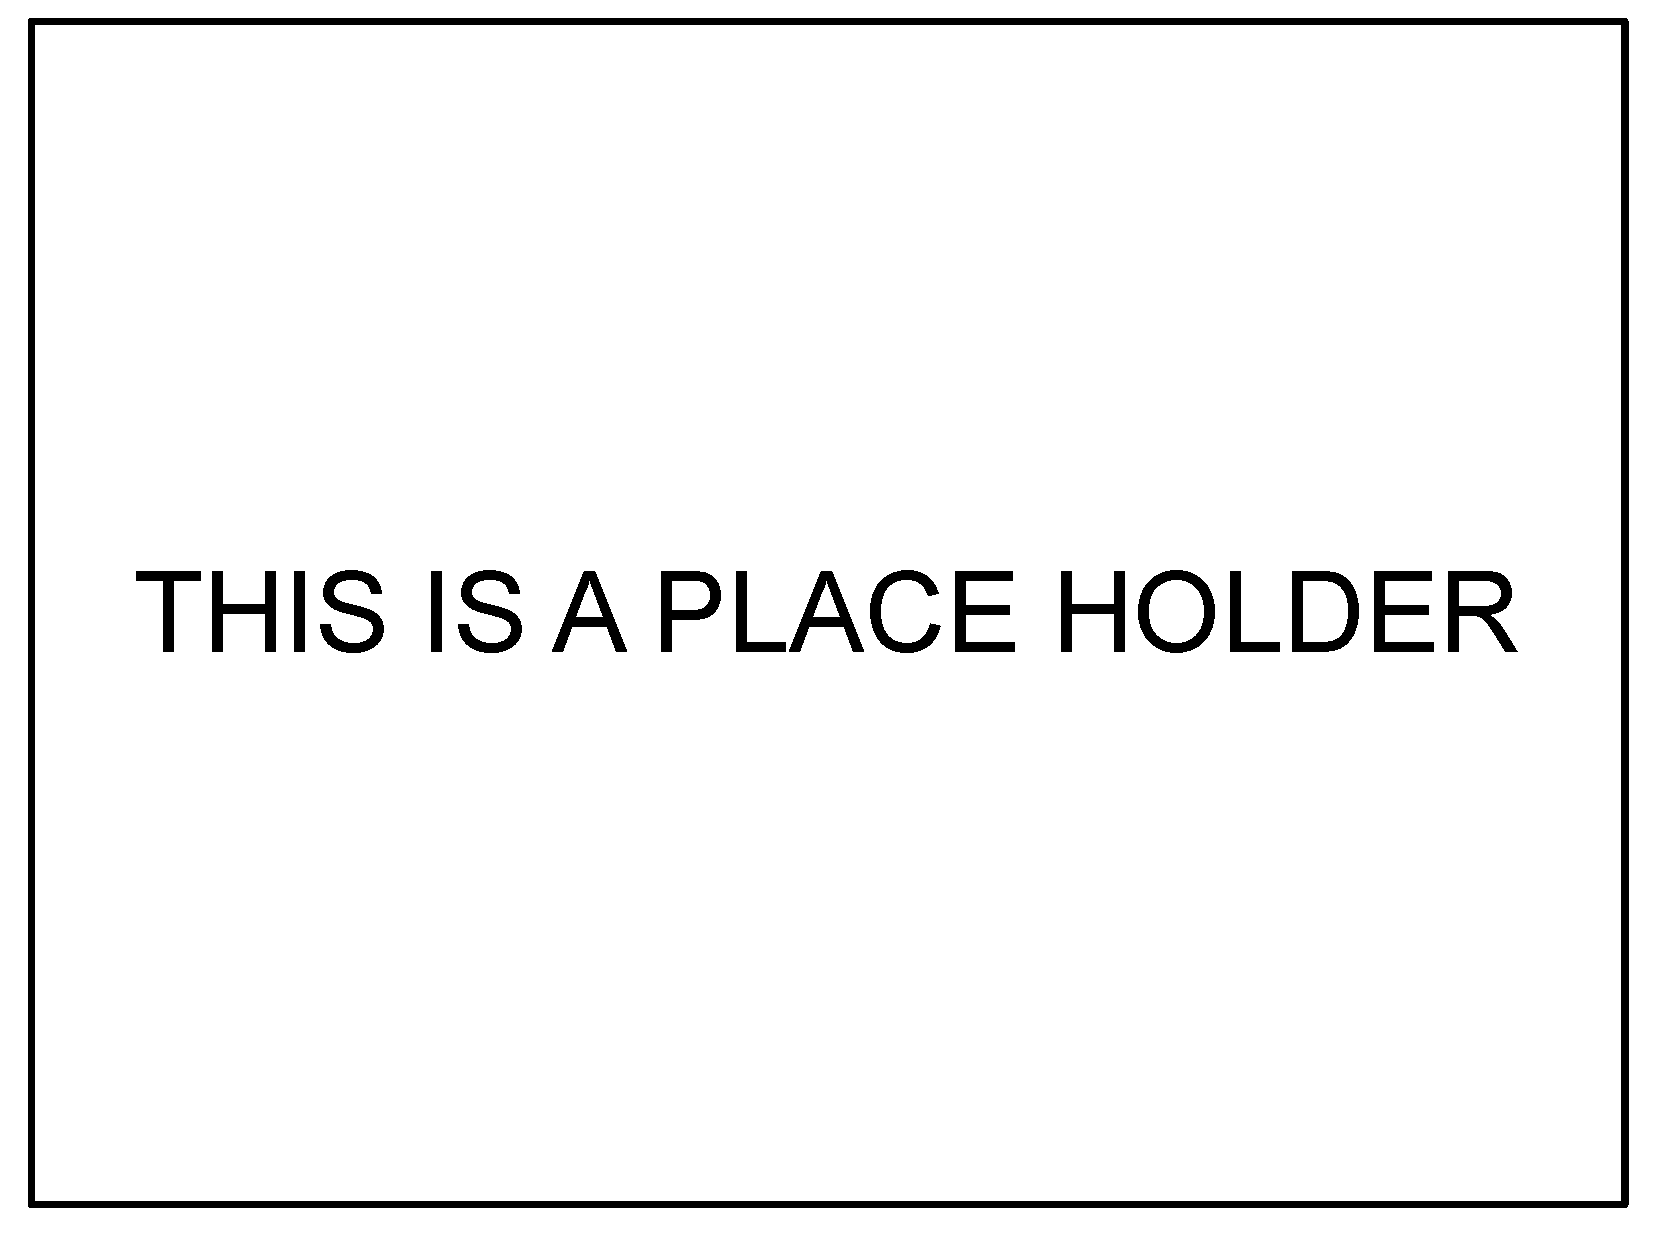
\includegraphics[width=0.3\textwidth]{figure/blank.pdf}
     }	
     \subfigure[]{		
            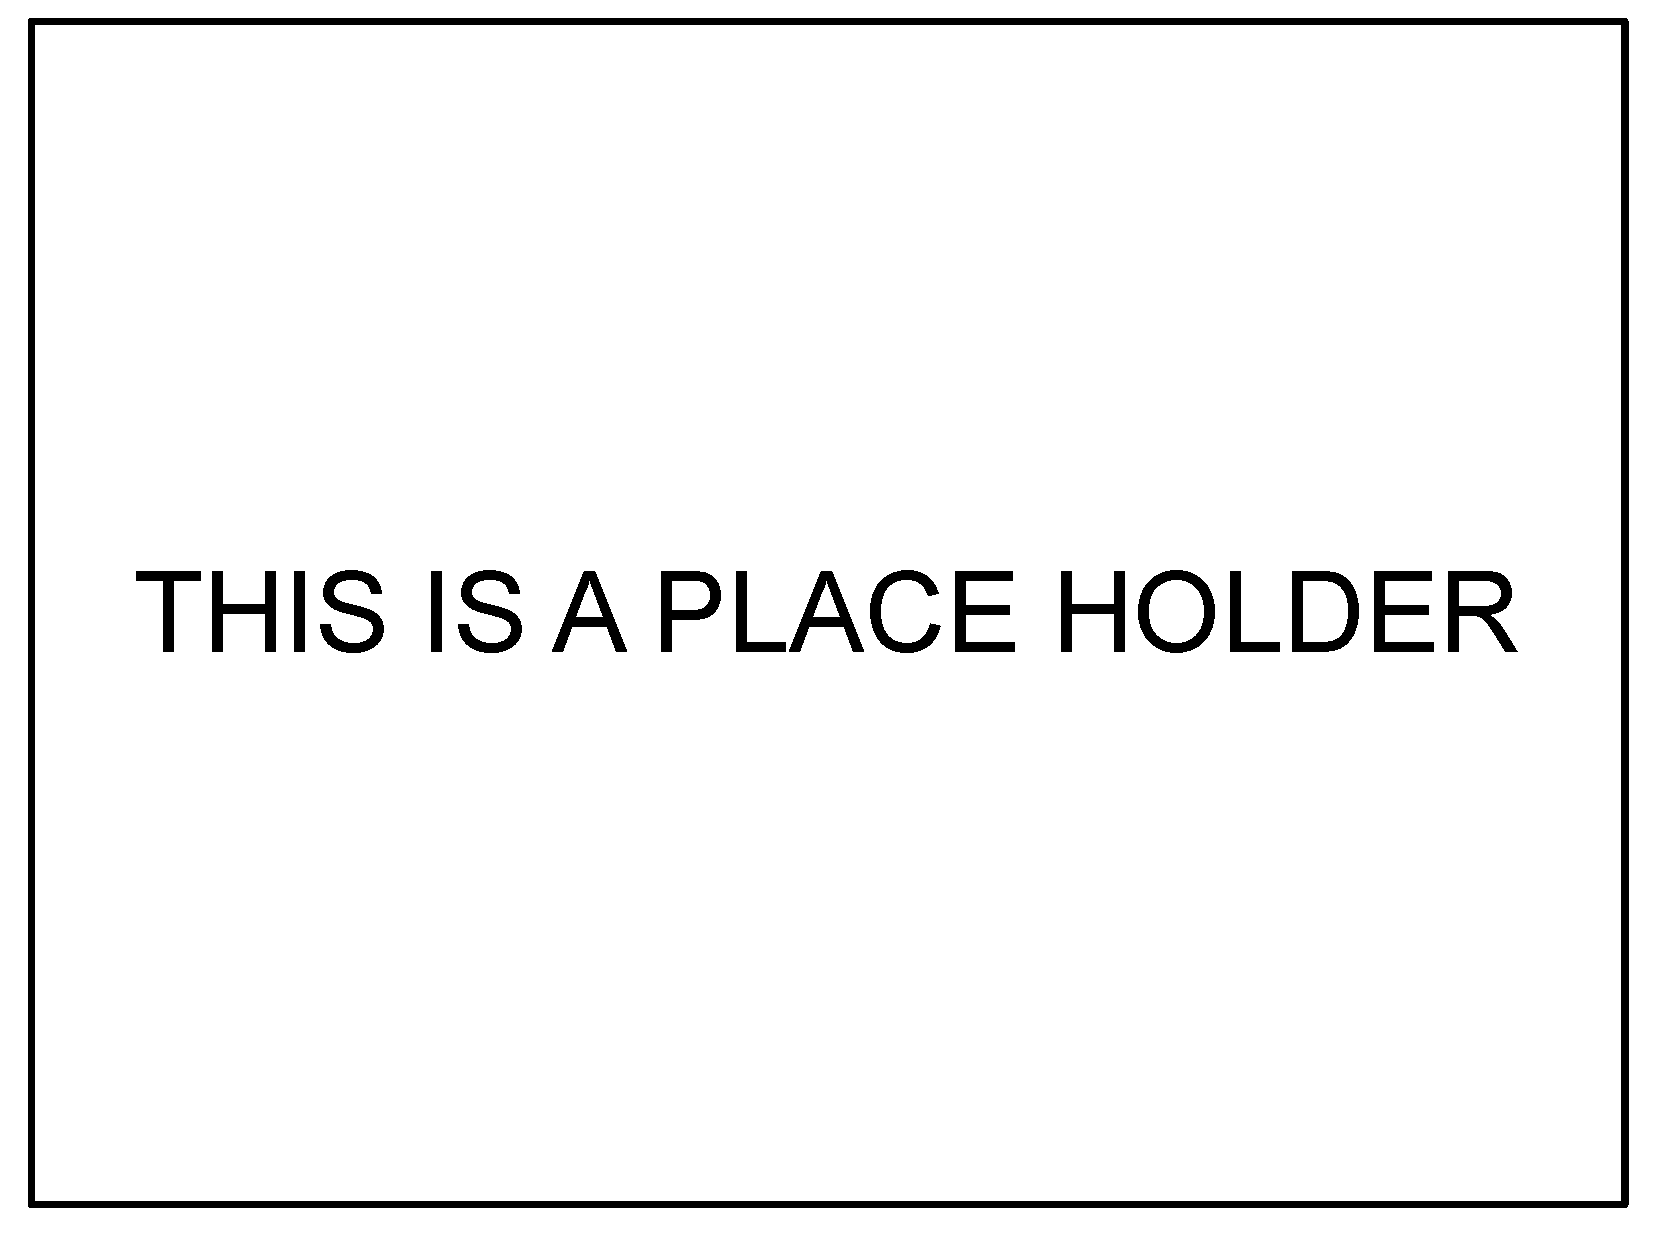
\includegraphics[width=0.3\textwidth]{figure/blank.pdf}
     }	
     \subfigure[]{		
            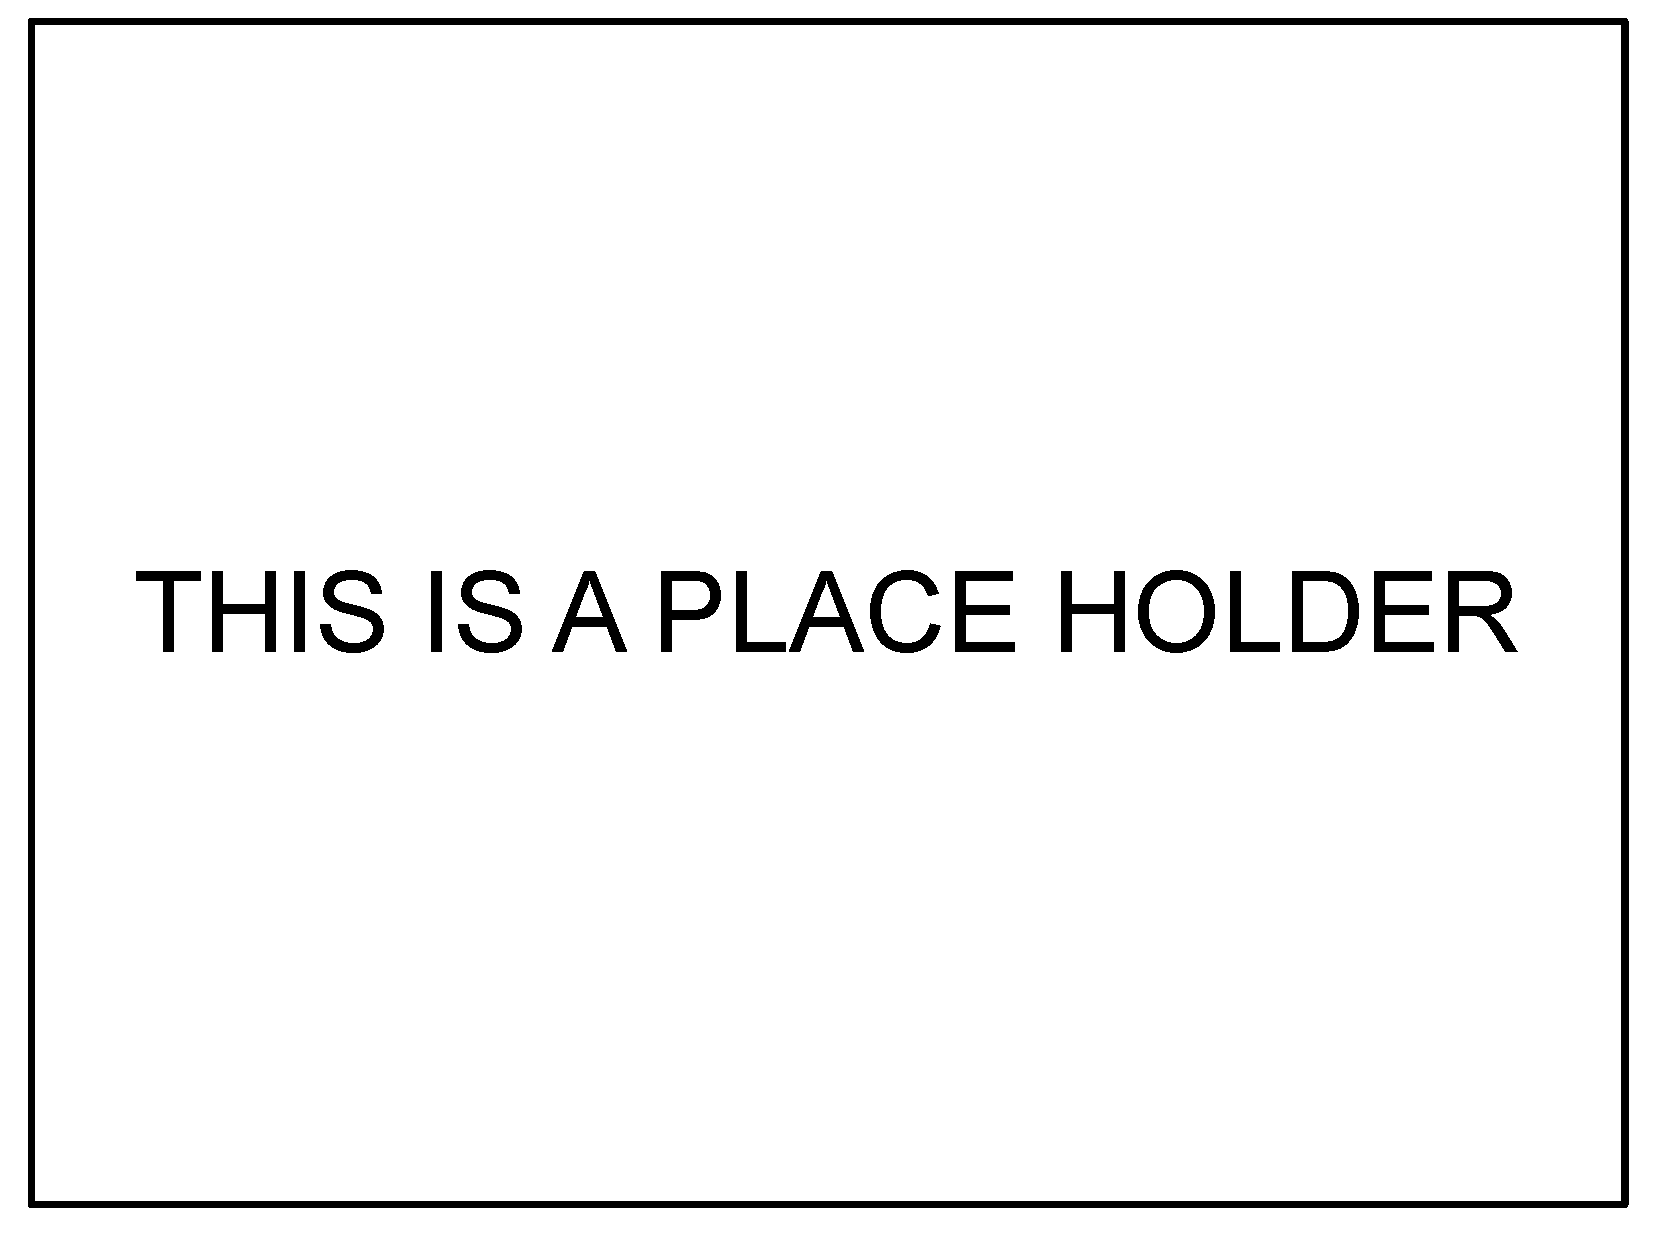
\includegraphics[width=0.3\textwidth]{figure/blank.pdf}
     }
     \end{center}
   \label{fig:couplings}
    \caption{Feynman diagrams for the couplings between one Higgs boson and two gauge bosons (a), two Higgs bosons and one gauge boson (b)
		and two Higgs bosons and two gauge bosons (c). Based on~\cite{Djuadi}. }
\end{figure}
Among these couplings, the most relevat for MSSM Higgs phenomenology is the trilinear couplings between two gauge bosons and one Higgs boson $V_{\mu}V_{\nu}H_i$,
in this case, since the photon is massless, there are no Higgs-$\gamma\gamma$ and Higgs-$Z\gamma$ couplings at tree level, CP-invariance also forbids $WWA$, $ZZA$
and $WZH^{\pm}$ couplings, for this case only the following couplings remains:
\begin{align} \label{eq:couplings}
Z_{\mu}Z_{\nu} h ~ :  ~ & ig_z M_Z \sin(\beta -\alpha) g_{\mu\nu},  &  Z_{\mu}Z_{\nu} H ~ : ~  ~    & ig_z M_Z \cos(\beta -\alpha) g_{\mu\nu} \\
W_{\mu}^+W_{\nu}^- h ~: ~&  ig_w M_W \sin(\beta -\alpha) g_{\mu\nu},  &  W_{\mu}^+W_{\nu}^- H ~ : ~ ~ & ig_w M_W \cos(\beta -\alpha) g_{\mu\nu}
\end{align}
The couplings of the neutral CP-even Higgs bosons $h$ and $H$ with pair of vector bosons are prortional to $ \sin(\beta -\alpha)$ and $\cos(\beta -\alpha)$
respectively, where $\cos(\beta -\alpha)$ is fixed at tree level following equation~\eqref{eq:couplings}. An interesting fenomenological consequence is
that, calling $G_{VVh}$ and $G_{VVH}$ a general   coupling between two vector bosons and one of the neutral CP-even Higgs bosons the following equation holds:
\begin{equation}\label{eq:couplingSM}
G^2_{VVh} +G^2_{VVH} = g^2_{VVH_{SM}}
\end{equation}
this means that the couplings with vector bosons for $h$ and $H$ respectively increase and decrease with $\tan\beta$, for
large value of $\tan\beta$, $h$ has SM-like couplings with vector bosons and $H$  decouple from them. For an overview of all the other
couplinq between vector boson and Higgs bosons, charged Higgs, trilinear and quartic coupling between Higgs bosons and couplings 
to SUSY particles refer to~\cite{Djuadi}.

The MSSM Higgs bosons couplings with isospin up-type $u$, and down-type $d$ fermions also depend on $\tan\beta$ and may be written
as follows:
\begin{align*}
G_{huu} ~\propto ~ & m_u [\sin(\beta - \alpha)  + \cot\beta \cos(\beta - \alpha)], & G_{hdd} ~\propto ~ & m_u [\sin(\beta - \alpha)  - \tan\beta \cos(\beta - \alpha)]\\
G_{Huu} ~\propto ~& m_u [\cos(\beta - \alpha)  - \cot\beta \sin(\beta - \alpha)], & G_{Hdd} ~\propto~  & m_d [\cos(\beta - \alpha)  + \tan\beta \sin(\beta - \alpha)]\\
G_{Auu} ~ \propto ~ & m_u  \cot\beta, & G_{Add} ~ \propto ~ & m_d \tan\beta 
\end{align*} 
Then the couplings of 




\subsection{MSSM Higgs Benchmark Scenarios}

\subsection{MSSM Higgs Production and Decay at the LHC}


